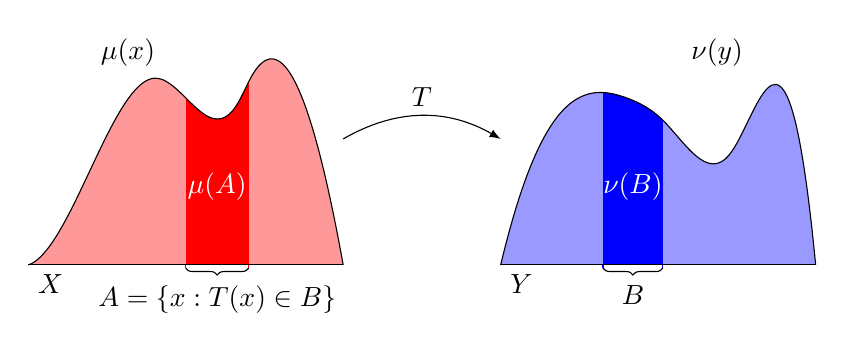
\begin{tikzpicture}[>=latex]
  % Define some colors for consistency
  \def\intensity{0.6}
  \definecolor{lightblue}{rgb}{\intensity, \intensity, 1}
  \definecolor{lightred}{rgb}{1, \intensity, \intensity}
  \def\pathA{(0.000, 0.000) .. controls (0.169, 0.054) and (0.338, 0.507) .. (0.507, 0.837)
   .. controls (0.606, 1.032) and (0.706, 1.184) .. (0.806, 1.186)
   .. controls (0.980, 1.189) and (1.154, 0.733) .. (1.328, 1.022)
   .. controls (1.359, 1.073) and (1.390, 1.147) .. (1.420, 1.201)
   .. controls (1.536, 1.402) and (1.651, 1.317) .. (1.766, 0.989)
   .. controls (1.844, 0.766) and (1.922, 0.432) .. (2.000, 0.000)}
  \def\pathB{(0.000, 0.000) .. controls (0.123, 0.515) and (0.246, 0.802) .. (0.368, 0.951)
   .. controls (0.518, 1.133) and (0.667, 1.112) .. (0.817, 1.054)
   .. controls (0.883, 1.028) and (0.948, 0.995) .. (1.014, 0.934)
   .. controls (1.161, 0.797) and (1.309, 0.516) .. (1.456, 0.705)
   .. controls (1.598, 0.886) and (1.740, 1.503) .. (1.882, 0.862)
   .. controls (1.921, 0.684) and (1.961, 0.408) .. (2.000, 0.000)}
  \def\Astart{1.0}
  \def\Aend{1.4}
  \def\Bstart{0.65}
  \def\Bend{1.03}
  \def\tickheight{0.02}
  \def\drawscale{2}
  \def\xlast{2cm}
  \def\boffset{\drawscale*3cm}
  \def\arrowoffset{0.8cm}

  % Left Blob (Initial Distribution)
  \begin{scope}[scale=\drawscale,red]
    \fill[lightred] \pathA;
    \begin{scope}
      \clip \pathA;
      \fill (\Astart, 0.0) rectangle (\Aend, 1.5);
    \end{scope}
    \draw[black] \pathA;
    \draw (\Astart, 0) -- (\Astart, -\tickheight) coordinate (A_start_tick);
    \draw (\Aend, 0) -- (\Aend, -\tickheight) coordinate (A_end_tick);
    \draw[black,decorate,decoration={brace,mirror}] (A_start_tick) -- (A_end_tick)
      node[midway,below=0.1cm] {$A = \left\{ x : T(x) \in B \right\}$};
    \node[anchor=north west,color=black] at (0.2*\xlast, 1.5cm) {$\mu(x)$};
    \node[anchor=center,color=white] at (0.5*\Astart + 0.5*\Aend, 0.5cm) {$\mu(A)$};
    \draw[black] (0,0) node [black,below right]{$X$} -- (\xlast,0);
  \end{scope}

  % Right Blob (Transformed Distribution)
  \begin{scope}[xshift=\boffset,scale=\drawscale,anchor=south west,color=blue]
    \fill[lightblue] \pathB;
    \begin{scope}
      \clip \pathB;
      \fill (\Bstart, 0.0) rectangle (\Bend, 1.5);
    \end{scope}
    \draw[black] \pathB;
    \draw (\Bstart, 0) -- (\Bstart, -\tickheight) coordinate (B_start_tick);
    \draw (\Bend, 0) -- (\Bend, -\tickheight) coordinate (B_end_tick);
    \draw[black,decorate,decoration={brace,mirror}] (B_start_tick) -- (B_end_tick)
      node[midway,below=0.1cm] {$B$};
    \node[anchor=north east,color=black] at (0.8*\xlast, 1.5cm) {$\nu(y)$};
    \node[anchor=center,color=white] at (0.5*\Bstart + 0.5*\Bend, 0.5cm) {$\nu(B)$};
    \draw[black] (0,0) node [black,below right]{$Y$} -- (\xlast,0);
  \end{scope}

  \draw[->, bend angle=30] (\drawscale*\xlast, \drawscale * \arrowoffset) to [bend left]
    node[above]{$T$} (\boffset, \drawscale * (\arrowoffset);

  % % Arrow
  % \draw[->, very thick] (6,0) to [bend right=30] (0,0);
  % \node at (3, 0.8) {$T$};
  %
  % % Labels for distributions
  % \node at (-1, -1) {$dv = \rho(q) dq$};
  % \node at (7, -1) {$du = \rho(x,t) dx$};
\end{tikzpicture}
